\documentclass[12pt]{article}

\usepackage{sbc-template}
\usepackage{graphicx,url}
\usepackage[utf8]{inputenc}
\usepackage[T1]{fontenc}
\usepackage[brazil]{babel}
\usepackage{booktabs}
\usepackage{amsmath}
\usepackage{multirow}
\usepackage{float}
\usepackage{array}
\usepackage{tikz}
\usetikzlibrary{shapes.geometric, arrows.meta, positioning}

\sloppy

\title{Detecção Automatizada de Estratégias \textit{Call2Go}:\\
       Pipeline \textit{Cross-Platform} para a Indústria Musical Brasileira}

\author{Lucas Fiori Magalhães Machado\inst{1}}

\address{Bacharelado em Ciência da Computação\\
  Pontifícia Universidade Católica de Minas Gerais (PUC Minas)\\
  Belo Horizonte -- MG, Brasil
  \email{lucasfmm54@gmail.com}
}

\begin{document}

\maketitle

% ============================================================
%  ABSTRACTS
% ============================================================
\begin{abstract}
This paper presents a multilayer regex-based system for automated detection
of \textit{Call2Go} strategies applied to 1,641 videos from 67 Brazilian
artists cross-platform persistent in Q1~2026 charts. Detection at video and
channel levels yields OR indicator ($518/1{,}641 = 31.6\%$) and AND indicator
($88/1{,}641 = 5.4\%$). Blind annotation of 91 adversarial videos yielded
Cohen's~$\kappa = 0.80$ (substantial) at channel level and $\kappa = 0.45$
(moderate) at video level. Mann-Whitney~U tests found no significant Call2Go
impact on YouTube views ($p=0.872$) or Spotify popularity ($p=1.000$).
Bidirectional Spearman confirmed unidirectional Spotify~$\to$~YouTube effect
($\rho=0.505$, $p<0.001$). Temporal lag analysis ($n=39$) showed YouTube
precedes chart entry by 882~days median, with publication volume in the 30
days prior as a significant predictor ($\rho=0.364$, $p=0.022$).
\end{abstract}

\begin{resumo}
Este trabalho apresenta um sistema automatizado baseado em \textit{regex}
multicamada para detecção de estratégias \textit{Call2Go}---chamadas de ação
em vídeos do YouTube direcionando ao Spotify---aplicado a 1.641 vídeos de 67
artistas brasileiros identificados como persistentes \textit{cross-platform}
nos \textit{charts} do Q1~2026 (Spotify Top~200~BR e YouTube Top~100~BR). A
detecção opera em dois níveis independentes: descrições de vídeo
(\textit{regex} multicamada) e perfis de canal (\textit{scraping} estruturado),
gerando os indicadores OR (vídeo \textit{ou} canal; métrica primária:
$518/1.641 = 31{,}6\%$) e AND (ambos simultaneamente; secundária:
$88/1.641 = 5{,}4\%$). Anotação às cegas de 91 vídeos adversariais resultou
em $\kappa = 0{,}80$ (concordância substancial) no nível de canal e
$\kappa = 0{,}45$ (moderada) no nível de vídeo, com acurácias de 90,1\% e
82,4\%, respectivamente. Testes Mann-Whitney~U não evidenciaram impacto
significativo do Call2Go nas visualizações do YouTube (OR: $U=280.705$,
$p=0{,}872$) nem na popularidade do Spotify (OR: $p=1{,}000$). Análise
bidirecional de Spearman confirmou efeito unidirecional Spotify~$\to$~YouTube
($\rho=0{,}505$, $p<0{,}001$). Análise de defasagem temporal ($n=39$
artistas) revelou que a atividade no YouTube precede a entrada nos
\textit{charts} em mediana de 882~dias (95\% dos artistas), com um preditor
significativo: volume de publicações nos 30~dias anteriores à estreia
($\rho=0{,}364$, $p=0{,}022$). O pipeline ETL de 15 etapas é inteiramente
reprodutível e determinístico.
\end{resumo}

% ============================================================
%  1. INTRODUÇÃO
% ============================================================
\section{Introdução}
\label{sec:intro}

A transformação digital da indústria fonográfica nas últimas duas décadas
reconfigurou profundamente as relações entre produção, distribuição e consumo
de música. O relatório anual da Federação Internacional da Indústria
Fonográfica (IFPI) registrou, em 2023, que as receitas provenientes de
serviços de \textit{streaming} responderam por 67\% do total global da música
gravada---uma inflexão histórica no modelo de negócios do
setor~\cite{ifpi2023}. O Brasil ocupa posição de destaque nesse cenário: é o
décimo maior mercado fonográfico do planeta e exibe taxas de crescimento em
\textit{streaming} que superam consistentemente a média
global~\cite{ifpi2023}. Dentro desse ecossistema, duas plataformas assumiram
protagonismo singular: o YouTube, maior repositório de vídeos do mundo e
principal canal de descoberta musical, e o Spotify, líder global em
\textit{streaming} de áudio com mais de 600 milhões de usuários ativos.

Nesse contexto, a estratégia denominada \textit{Call2Go} emergiu como prática
amplamente difundida na indústria musical brasileira. O termo descreve qualquer
elemento inserido na descrição de um vídeo do YouTube---seja um hiperlink
direto ao Spotify, seja uma chamada textual de ação
(\textit{call-to-action})---com o propósito explícito de redirecionar o
espectador para a plataforma de \textit{streaming} de áudio. A lógica
subjacente fundamenta-se na hipótese de que a audiência conquistada no YouTube,
plataforma de acesso gratuito e onipresente, pode ser convertida em assinantes
ou ouvintes recorrentes no Spotify, cuja monetização por \textit{stream} é
diretamente mais vantajosa para artistas e distribuidoras~\cite{wlomert2016}.

A investigação científica sobre as dinâmicas \textit{cross-platform} na música
digital ainda se encontra em estágio formativo~\cite{aguiar2021}. Os estudos
existentes concentram-se predominantemente em análises agregadas de mercado ou
em fenômenos observados em plataformas isoladas, sem abordar
sistematicamente os mecanismos de transferência de audiência entre YouTube e
Spotify~\cite{napoli2010}. Ademais, a ausência de ferramentas automatizadas
validadas para a detecção de Call2Go em larga escala representa um obstáculo
metodológico significativo: a anotação manual de grandes \textit{corpora} é ao
mesmo tempo impraticável operacionalmente e sujeita a vieses de subjetividade
entre anotadores. A lacuna identificada é, portanto, dupla: \textbf{empírica},
pela ausência de evidências sobre a eficácia da estratégia no mercado
brasileiro, e \textbf{metodológica}, pela inexistência de instrumentos
confiáveis para sua detecção automatizada em escala.

Este trabalho endereça diretamente essa lacuna ao propor, implementar e
validar um sistema automatizado de detecção de Call2Go baseado em expressões
regulares multicamada. O foco central da investigação recai sobre a
\textbf{confiabilidade metodológica} da ferramenta desenvolvida, mensurada
por meio de um protocolo de validação cruzada com design adversarial e anotação
humana às cegas. Secundariamente, os dados coletados são empregados para
testar hipóteses sobre o impacto estatístico do Call2Go no engajamento em
ambas as plataformas, investigar a direcionalidade da relação entre métricas
do YouTube e do Spotify, e analisar a defasagem temporal entre a atividade
de publicação no YouTube e a entrada dos artistas nos \textit{charts}.

As principais contribuições são: (i)~um sistema determinístico e auditável de
detecção em dois níveis com operadores OR e AND; (ii)~um protocolo de validação
adversarial às cegas com Kappa de Cohen e IC~95\% \textit{bootstrap};
(iii)~um pipeline ETL reprodutível de 15 etapas integrando YouTube, Spotify e
Last.fm; e (iv)~análise de defasagem temporal entre atividade no YouTube e
\textit{charts} Spotify para artistas brasileiros.

O artigo está organizado da seguinte forma: a Seção~\ref{sec:literatura}
revisa a literatura relevante; a Seção~\ref{sec:objetivos} apresenta objetivos
e hipóteses; a Seção~\ref{sec:metodologia} detalha o pipeline; a
Seção~\ref{sec:resultados} expõe os resultados; e a
Seção~\ref{sec:conclusao} apresenta as conclusões e trabalhos futuros.

% ============================================================
%  2. REVISÃO DA LITERATURA
% ============================================================
\section{Revisão da Literatura}
\label{sec:literatura}

\subsection{Marketing Digital e \textit{Cross-Platform} na Música}

A digitalização da cadeia produtiva musical transformou não apenas os canais
de distribuição, mas os modelos de relacionamento entre artistas, intermediários
e audiências. Aguiar e Waldfogel~\cite{aguiar2021} documentaram empiricamente
que as plataformas de distribuição digital alteraram as dinâmicas de
promoção, deslocando poder das grandes gravadoras para distribuidoras
independentes e, em determinados contextos, para os próprios artistas. YouTube
e Spotify exercem funções complementares na jornada de consumo musical: o
YouTube opera primariamente como plataforma de descoberta e videoconsumo, ao
passo que o Spotify consolida o consumo recorrente em forma de \textit{stream}
contabilizável~\cite{wlomert2016}.

As estratégias de \textit{cross-platform marketing} na música seguem uma
lógica de funil: o conteúdo audiovisual no YouTube atua como ponto de entrada
de alta viralidade e baixo custo de aquisição, enquanto as plataformas de
\textit{streaming} de áudio representam o destino de conversão de valor.
Wlömert e Papies~\cite{wlomert2016} demonstraram que a entrada do Spotify no
mercado gerou efeitos assimétricos sobre as receitas da indústria, sem abordar
especificamente os mecanismos de direcionamento interplataforma originados no
YouTube. Napoli~\cite{napoli2010} argumenta que a fragmentação das audiências
digitais impõe novos desafios de medição e atribuição de causalidade entre
plataformas.

O mercado brasileiro apresenta características estruturais que potencializam
a relevância da questão: o país figura consistentemente entre os maiores
mercados do YouTube por volume de horas assistidas~\cite{ifpi2023} e
experimenta uma das transições mais rápidas do mundo de consumo musical
gratuito para \textit{streaming} pago, com artistas do sertanejo, pagode e
funk acumulando bilhões de visualizações enquanto buscam migrar sua base para
plataformas remuneradas.

\subsection{Análise Automatizada de Conteúdo em Plataformas Digitais}

A análise de conteúdo como método científico foi sistematizada por
Krippendorff~\cite{krippendorff2004}, que a define como ``uma técnica de
pesquisa para fazer inferências replicáveis e válidas a partir de textos para
os contextos de seu uso''. No campo da recuperação de informação musical
(\textit{Music Information Retrieval}, MIR), Schedl et
al.~\cite{schedl2014} catalogaram as principais abordagens de análise
automatizada de metadados musicais, incluindo o processamento de texto
associado a conteúdo audiovisual.

Sistemas baseados em regras, como o motor \textit{regex} proposto neste
trabalho, caracterizam-se por alta interpretabilidade, custo computacional
negligenciável e comportamento determinístico---propriedades especialmente
valiosas em contexto acadêmico, onde reprodutibilidade e auditabilidade
constituem requisitos metodológicos~\cite{salganik2019}. Friedl~\cite{friedl2006}
documenta extensivamente a expressividade e os limites das expressões regulares
como ferramenta de \textit{pattern matching}. Celma~\cite{celma2010} destacou
que a esparsidade e o ruído inerentes aos metadados de vídeo dificultam a
extração consistente de informações estruturadas, fenômeno particularmente
agudo em descrições do YouTube, onde URLs encurtadas e redirecionadores de
terceiros ocultam o destino final dos links.

A distinção entre menções narrativas e chamadas de ação constitui um dos
problemas mais recorrentes na análise automatizada de descrições de vídeo.
Um artista pode mencionar o Spotify em frases como ``alcançamos 10 milhões de
\textit{plays} no Spotify'' (menção narrativa, não-Call2Go) ou ``ouça no
Spotify'' (chamada de ação, Call2Go). Sistemas baseados em
\textit{keyword matching} simples tratam ambos os casos de forma idêntica,
produzindo falsos positivos que comprometem a validade da análise.

\subsection{Confiabilidade em Sistemas de Classificação Automatizada}

A avaliação da confiabilidade de sistemas de classificação automatizada em
relação a referências humanas constitui problema central em pesquisa
computacional. O índice kappa de Cohen~\cite{cohen1960} representa a medida
pioneira de concordância entre dois anotadores além do nível esperado pelo
acaso. Fleiss~\cite{fleiss1971} estendeu o índice para múltiplos anotadores.
Landis e Koch~\cite{landis1977} estabeleceram a escala interpretativa
amplamente adotada: $\kappa < 0{,}20$ (fraca), $0{,}21$--$0{,}40$ (razoável),
$0{,}41$--$0{,}60$ (moderada), $0{,}61$--$0{,}80$ (substancial) e
$0{,}81$--$1{,}00$ (quase perfeita).

Salganik~\cite{salganik2019} argumenta que pesquisas computacionais em
ciências sociais enfrentam um dilema entre escala e validade: métodos
automatizados permitem analisar \textit{corpora} de milhões de registros, mas
sua validade depende de etapas de verificação humana sobre amostras. O design
adversarial da validação---em que os casos selecionados desafiam
especificamente o detector, ao invés de uma amostragem aleatória---maximiza
o rigor metodológico ao forçar o sistema a demonstrar robustez nos casos mais
difíceis.

A Tabela~\ref{tab:literatura} sintetiza comparativamente as principais
abordagens para análise automatizada de conteúdo em plataformas digitais.

\begin{table}[H]
\centering
\caption{Comparativo de abordagens para análise automatizada de conteúdo.}
\label{tab:literatura}
\renewcommand{\arraystretch}{1.1}
\begin{tabular}{@{}lllll@{}}
\toprule
\textbf{Abordagem} & \textbf{Mecanismo} & \textbf{Escala} &
\textbf{Validação} & \textbf{Limitação} \\
\midrule
Anotação manual         & Humano              & Pequena & Alta   & Não escalável \\
\textit{Keyword match}  & Palavras-chave      & Grande  & Baixa  & Alta taxa FP \\
\textit{Regex} básico   & Padrões fixos       & Grande  & Média  & Sensível ao contexto \\
\textit{Regex} multicamada & Hierarquia de regras & Grande & Alta & Domínio-específico \\
ML supervisionado       & Classificador       & Grande  & Média  & Exige corpus rotulado \\
NLP profundo            & Transformers        & Grande  & Alta   & Alto custo computacional \\
\bottomrule
\end{tabular}
\end{table}

% ============================================================
%  3. OBJETIVOS DA PESQUISA
% ============================================================
\section{Objetivos da Pesquisa}
\label{sec:objetivos}

\subsection{Objetivo Geral}

Desenvolver, implementar e validar um sistema automatizado baseado em
expressões regulares para a detecção de estratégias Call2Go em vídeos do
YouTube, aplicado ao corpus de artistas brasileiros persistentes
\textit{cross-platform} nos \textit{charts} Q1~2026, e avaliar sua
confiabilidade metodológica por meio de protocolo de validação cruzada com
anotação humana às cegas, além de analisar o impacto estatístico da
estratégia em métricas de engajamento e a relação temporal entre atividade
no YouTube e entrada em \textit{charts} Spotify.

\subsection{Objetivos Específicos}

\begin{enumerate}
  \item Construir uma base de artistas reprodutível derivada da interseção de
    \textit{charts} semanais Spotify Top~200~BR e YouTube Top~100~BR ao longo
    das 13 semanas do Q1~2026, com critério de persistência em ambas as
    plataformas.

  \item Coletar e estruturar um corpus de vídeos do YouTube (30 mais
    visualizados por artista) via YouTube Data API~v3~\cite{youtubeapi2024},
    métricas do Spotify via Spotify Web API~\cite{spotifyapi2024} e dados do
    Last.fm via Last.fm API~\cite{lastfmapi2024}.

  \item Desenvolver um motor de detecção Call2Go em dois níveis analíticos
    independentes (vídeo e canal), com operadores lógicos OR (primário) e AND
    (sub-análise), capaz de distinguir entre links diretos, redirecionadores de
    terceiros e menções textuais implícitas, com filtragem automática de
    menções narrativas.

  \item Construir um \textit{ground truth} humano às cegas sobre 91 vídeos
    adversariais e avaliar a confiabilidade do detector reportando acurácia,
    Kappa de Cohen com IC~95\% \textit{bootstrap}, precisão, \textit{recall}
    e F1-score por nível analítico.

  \item Testar as hipóteses $H_2$ e $H_3$ via Mann-Whitney~U ($\alpha = 0{,}05$)
    para as métricas OR e AND, e conduzir análise bidirecional de Spearman
    entre métricas YouTube e Spotify ($\alpha = 0{,}10$).

  \item Realizar análise de defasagem temporal ($H_4$) entre a data de
    publicação de vídeos no YouTube e a data de entrada dos artistas nos
    \textit{charts} Spotify BR, identificando preditores de desempenho nos
    \textit{charts}.

  \item Consolidar um pipeline ETL reprodutível de 15 etapas em Python~3.12
    \cite{python2024}, integrando pandas~\cite{mckinney2010},
    SciPy~\cite{virtanen2020} e SQLite, com 30 artefatos de saída
    verificáveis.
\end{enumerate}

\subsection{Hipóteses de Pesquisa}

\begin{itemize}
  \item[$H_0$] O detector automatizado não apresenta concordância
    estatisticamente significativa com a classificação humana (acurácia
    $< 85\%$).
  \item[$H_1$] O detector atinge acurácia $\geq 85\%$ em relação ao
    \textit{ground truth} humano, validando a abordagem como metodologicamente
    confiável.
  \item[$H_2$] Vídeos com Call2Go~OR apresentam volume de visualizações
    significativamente maior no YouTube do que vídeos sem a estratégia.
  \item[$H_3$] A presença de Call2Go~OR está positivamente associada a maior
    pontuação de popularidade no Spotify.
  \item[$H_4$] A atividade de publicação no YouTube antecede temporalmente a
    entrada do artista nos \textit{charts} Spotify, e a intensidade dessa
    atividade pré-entrada correlaciona-se com o desempenho nos \textit{charts}.
\end{itemize}

% ============================================================
%  4. METODOLOGIA
% ============================================================
\section{Metodologia}
\label{sec:metodologia}

A Figura~\ref{fig:pipeline} apresenta o pipeline ETL e de análise, composto
por 15 etapas sequenciais organizadas em cinco blocos funcionais.

\begin{figure}[H]
\centering
\begin{tikzpicture}[
    node distance=0.85cm,
    box/.style={rectangle, draw=black!70, fill=gray!10, text width=11cm,
                text centered, minimum height=0.65cm, font=\small,
                rounded corners=2pt},
    abox/.style={rectangle, draw=green!60!black, fill=green!8, text width=11cm,
                 text centered, minimum height=0.65cm, font=\small,
                 rounded corners=2pt},
    vbox/.style={rectangle, draw=blue!60, fill=blue!8, text width=11cm,
                 text centered, minimum height=0.65cm, font=\small,
                 rounded corners=2pt},
    arr/.style={-{Stealth}, thick, draw=black!60}
]
\node[box]  (s1) {Etapas 1--5: Coleta (Artistas, YouTube, Spotify, Last.fm, \textit{Scraping} de Canais)};
\node[box,  below of=s1] (s2) {Etapa 6: Detecção Call2Go --- \textit{Regex} Multicamada (OR + AND)};
\node[box,  below of=s2] (s3) {Etapa 7: \textit{Data Warehouse} SQLite (6 tabelas, \textit{star schema})};
\node[abox, below of=s3] (s4) {Etapas 8--11: EDA + Mann-Whitney + Cross-Platform + Last.fm Bridge};
\node[abox, below of=s4] (s5) {Etapa 12: Validação Bidirecional YouTube $\leftrightarrow$ Spotify};
\node[abox, below of=s5] (s6) {Etapas 13--15: Datas Spotify + Ranking Fusion + Análise Temporal};
\node[vbox, below of=s6] (s7) {[Validação Independente] 91 vídeos adversariais, anotação às cegas};
\draw[arr] (s1) -- (s2);
\draw[arr] (s2) -- (s3);
\draw[arr] (s3) -- (s4);
\draw[arr] (s4) -- (s5);
\draw[arr] (s5) -- (s6);
\draw[arr] (s6) -- (s7);
\end{tikzpicture}
\caption{Pipeline ETL e de validação (15 etapas). Cinza: extração/carga;
verde: análise estatística; azul: validação cruzada independente.}
\label{fig:pipeline}
\end{figure}

\subsection{Construção da Base de Artistas e Coleta de Dados}

A construção da base de artistas adota um critério de persistência
\textit{cross-platform}: foram considerados os artistas presentes em pelo
menos uma semana dos \textit{charts} Spotify Top~200~BR \textbf{e} YouTube
Top~100~BR ao longo das 13 semanas do Q1~2026 (janeiro a março). Após
deduplicação e correspondência de identidades entre plataformas por
normalização de nomes (NFKD, minúsculas, sem pontuação), foram identificados
67 artistas brasileiros persistentes. A lista de artistas é derivável
diretamente dos \textit{charts} estáticos armazenados no repositório,
garantindo reprodutibilidade.

Para o YouTube, a coleta usa o endpoint \texttt{playlistItems.list}
(custo: 1 unidade de cota por chamada), acessando a \textit{uploads playlist}
de cada canal ao substituir o prefixo \texttt{UC} por \texttt{UU} para
recuperar até 200 vídeos, ordenando localmente por \texttt{viewCount} e
selecionando os 30 mais visualizados~\cite{youtubeapi2024}. Essa abordagem
reduz o consumo estimado de cota em ${\sim}89\%$ em relação ao
\texttt{search.list} (100 unidades/chamada). Os 30 vídeos de cada um dos
67 artistas totalizam \textbf{1.641 vídeos} analisados.

Canais do tipo OAC (\textit{Official Artist Channel}), gerados
automaticamente pelo YouTube por fusão de canais, foram tratados com busca
automática do canal oficial principal do artista, uma vez que não possuem
links personalizados na aba ``Sobre''.

As métricas do Spotify foram coletadas via Spotify Web
API~\cite{spotifyapi2024} com autenticação \textit{Client Credentials}
(OAuth~2.0), com \textit{snapshot} de popularidade e seguidores capturado em
22 de abril de 2026. O campo \texttt{popularity} é um índice algorítmico de
0 a 100, calculado pela plataforma com base em recência e frequência de
\textit{streams}. Métricas do Last.fm foram coletadas via Last.fm
API~\cite{lastfmapi2024} para os 67 artistas, cobrindo \textit{listeners},
\textit{scrobbles} e \textit{top tracks}, além dos \textit{charts} brasileiros
Top~200 artistas e faixas.

\subsection{\textit{Scraping} Estruturado de Links de Canal}

A aba ``Sobre'' dos canais do YouTube expõe links externos estruturados que
\textbf{não são acessíveis pela YouTube Data API~v3}. Essa lacuna é
metodologicamente crítica: os links do Spotify inseridos na seção pública
do canal constituem a fonte de detecção para 25,0\% dos vídeos do corpus. Um
\textit{scraper}~\cite{mitchell2018} foi desenvolvido em duas fases: a Fase~1
extrai o objeto JSON \texttt{ytInitialData} da página principal do canal e
busca o elemento \texttt{channelExternalLinkViewModel}; a Fase~2, como
\textit{fallback}, acessa a subpágina \texttt{/about} e aplica
\textit{regex} na bio do canal.

Um tratamento especial foi implementado para a decodificação de caracteres
\texttt{\textbackslash u0026} (sequência de escape Unicode para ``\&''), cuja
ausência de decodificação resultava em URLs de redirecionamento truncadas e
perda de detecções válidas. O módulo opera em modo \textit{cache-first} por
padrão, garantindo reprodutibilidade entre execuções sem dependência de
disponibilidade de página.

\subsection{Motor de Detecção Call2Go: \textit{Regex} Multicamada}
\label{sec:detector}

O motor de detecção opera em dois níveis analíticos independentes, cada um
com uma hierarquia de regras:

\textbf{Nível Vídeo} (descrição textual): quatro camadas de regras detectam
(R1)~links diretos a domínios proprietários do Spotify
(\texttt{open.spotify.com}, \texttt{spoti.fi}, \texttt{sptfy.com});
(R2)~\textit{labeled redirects}, detectando a coexistência de um domínio de
redirecionamento (\texttt{lnk.to}, \texttt{bit.ly}, \texttt{smarturl.it})
com o rótulo ``spotify'' a uma distância máxima de 50 caracteres
(\texttt{.\{0,50\}}); (R3)~token \texttt{spotify}/\texttt{sptfy} no
\textit{path} da URL; e (R4)~chamadas de ação verbais sem link, cobrindo
construções em português:
$\texttt{ou[çc]a\textbackslash b.\{0,50\}\textbackslash bspotify}$,
$\texttt{dispon[ií]vel\textbackslash b.\{0,30\}\textbackslash bspotify}$,
$\texttt{\textbackslash bstream\textbackslash b.\{0,50\}\textbackslash bspotify}$
e variações. O operador \texttt{.\{0,N\}} substituiu o operador guloso
\texttt{.*} para evitar \textit{matches cross-sentence} em bios extensas.

\textbf{Nível Canal} (links scrapeados + fallback bio): aplica as mesmas
regras R1--R3 sobre os links estruturados da aba ``Sobre'' e sobre a bio do
canal, capturando padrões como \texttt{"Spotify - bit.ly/..."} não expostos
pela API.

\textbf{Filtragem de menções narrativas}: antes de qualquer regra de
detecção, o texto é submetido a um pré-filtro que invalida seis padrões de
menção contextual sem intenção de CTA, incluindo
\texttt{chart\textbackslash w*\textbackslash s+(?:do|no)\textbackslash s+spotify},
variações de \textit{top}~$N$, posição numérica em ranking e referências a
estatísticas de \textit{streams} (``milhões de plays no Spotify'').

\textbf{Combinação lógica}: as duas camadas geram métricas complementares:
(i)~\textbf{OR} (\textit{primary}): vídeo \textit{ou} canal apresentam Call2Go
--- captura qualquer articulação da estratégia;
(ii)~\textbf{AND} (\textit{secondary}): vídeo \textit{e} canal apresentam
Call2Go simultaneamente --- captura a forma mais integrada e intencional de
adoção.

\subsection{\textit{Data Warehouse} e Análises Estatísticas}

Os dados coletados são carregados em um \textit{data warehouse} SQLite com
\textit{star schema} de 6 tabelas: \texttt{dim\_artist},
\texttt{fact\_yt\_videos} (com colunas \texttt{has\_call2go} e
\texttt{has\_call2go\_or}), \texttt{fact\_spotify\_metrics},
\texttt{fact\_lastfm\_metrics}, \texttt{fact\_lastfm\_chart\_artists} e
\texttt{fact\_lastfm\_chart\_tracks}. O banco é reconstruído integralmente a
cada execução (\textit{batch rebuild}), garantindo consistência entre dados
brutos e o artefato analítico.

Para os testes $H_2$ e $H_3$, o Mann-Whitney~U foi selecionado por ser não
paramétrico, adequado para amostras de tamanhos distintos e robusto a
\textit{outliers}~\cite{mann1947}. Para a análise bidirecional e temporal, a
correlação de Spearman~\cite{spearman1904} foi adotada pela capacidade de
detectar relações monotônicas não lineares entre as métricas das plataformas.
O nível de significância é $\alpha = 0{,}05$ para $H_2$ e $H_3$, e
$\alpha = 0{,}10$ para a análise bidirecional (reconhecendo o tamanho amostral
a nível de artista, $N = 67$).

A análise temporal ($H_4$) define três janelas de observação relativas à
data de entrada de cada artista no \textit{chart} Spotify: $[-30; 0]$,
$[-90; 0]$ e o período total de publicação no YouTube. A defasagem
(\textit{lag}) é calculada como a diferença em dias entre o primeiro vídeo do
artista no YouTube e sua primeira aparição no \textit{chart} Spotify BR
Q1~2026. O método de Ranking Fusion emprega \textit{Reciprocal Rank
Fusion}~\cite{cormack2009} com normalização por número de semanas, integrando
\textit{charts} do Spotify e YouTube em um \textit{score} combinado.

\subsection{Protocolo de Validação Cruzada}

A validação adota \textbf{design adversarial} para maximizar o rigor
metodológico. Em vez de amostrar aleatoriamente do corpus, foram
selecionados 91 vídeos que desafiam especificamente o detector: casos
limítrofes com redirecionadores de terceiros, emojis, URLs codificadas,
textos ambíguos entre CTA e menção narrativa, e perfis de canal com formato
incomum. A anotação foi conduzida às \textbf{cegas}: o anotador humano
classificou cada vídeo sem visualizar a saída do sistema automatizado,
eliminando o viés de confirmação presente em protocolos circulares.

As métricas reportadas são: acurácia, precisão, \textit{recall}, F1-score e
Kappa de Cohen com IC~95\% via \textit{bootstrap} ($B = 10.000$ reamostras)
\cite{cohen1960}. A validação é conduzida em dois níveis independentes:
\textbf{Nível Vídeo} (detector restrito à descrição textual) e \textbf{Nível
Canal} (detector restrito ao perfil do canal). Esse design, que
desacopla os dois níveis, permite identificar onde o sistema é forte e onde
apresenta margens de melhoria, com maior valor diagnóstico do que uma
avaliação combinada.

% ============================================================
%  5. RESULTADOS
% ============================================================
\section{Resultados e Análises}
\label{sec:resultados}

\subsection{Distribuição das Detecções de Call2Go}

A execução do motor de detecção sobre o corpus completo de 1.641 vídeos
produziu os resultados descritos na Tabela~\ref{tab:deteccao}. A métrica
primária OR identifica 518 vídeos (31,6\%) com Call2Go em ao menos um nível;
a sub-análise AND identifica 88 vídeos (5,4\%) com Call2Go simultâneo em
ambos os níveis.

\begin{table}[H]
\centering
\caption{Distribuição das detecções por nível e lógica combinada
(corpus: 1.641 vídeos, 67 artistas).}
\label{tab:deteccao}
\renewcommand{\arraystretch}{1.2}
\begin{tabular}{@{}llrr@{}}
\toprule
\textbf{Nível / Métrica} & \textbf{Lógica} & \textbf{Vídeos} & \textbf{\%} \\
\midrule
Nível Vídeo  (descrição)          & ---                 & 196   & 11,9 \\
Nível Canal  (scraping)           & ---                 & 410   & 25,0 \\
\midrule
\textbf{OR (métrica primária)}    & vídeo \textit{ou} canal & \textbf{518} & \textbf{31,6} \\
AND (sub-análise)                 & vídeo \textit{e} canal  & 88   &  5,4 \\
Sem Call2Go (OR)                  & ---                 & 1.123 & 68,4 \\
\midrule
\textbf{Total}                    & ---                 & \textbf{1.641} & \textbf{100,0} \\
\bottomrule
\end{tabular}
\end{table}

A decomposição por nível revela que o canal é a fonte dominante: 25,0\% dos
vídeos têm Call2Go detectado via \textit{scraping} da aba ``Sobre'',
confirmando a imprescindibilidade do módulo de scraping. Apenas 11,9\% têm
Call2Go na descrição individual, reforçando que a prática dominante é inserir
o link no perfil do canal---válido para \textit{todos} os vídeos do artista
---e não em cada descrição separadamente. Os 5,4\% de vídeos AND representam
artistas que adotam a estratégia simultaneamente nos dois níveis, a forma
mais integrada de Call2Go.

\subsection{Análise Exploratória de Dados (EDA)}

A análise exploratória confrontou as distribuições de \texttt{view\_count}
para os grupos Call2Go~OR ($n = 518$) e sem Call2Go ($n = 1.123$). Em ambos,
a distribuição é altamente assimétrica à direita, com cauda longa de vídeos
virais, conforme evidenciado na Figura~\ref{fig:boxplot}.

\begin{figure}[H]
\centering
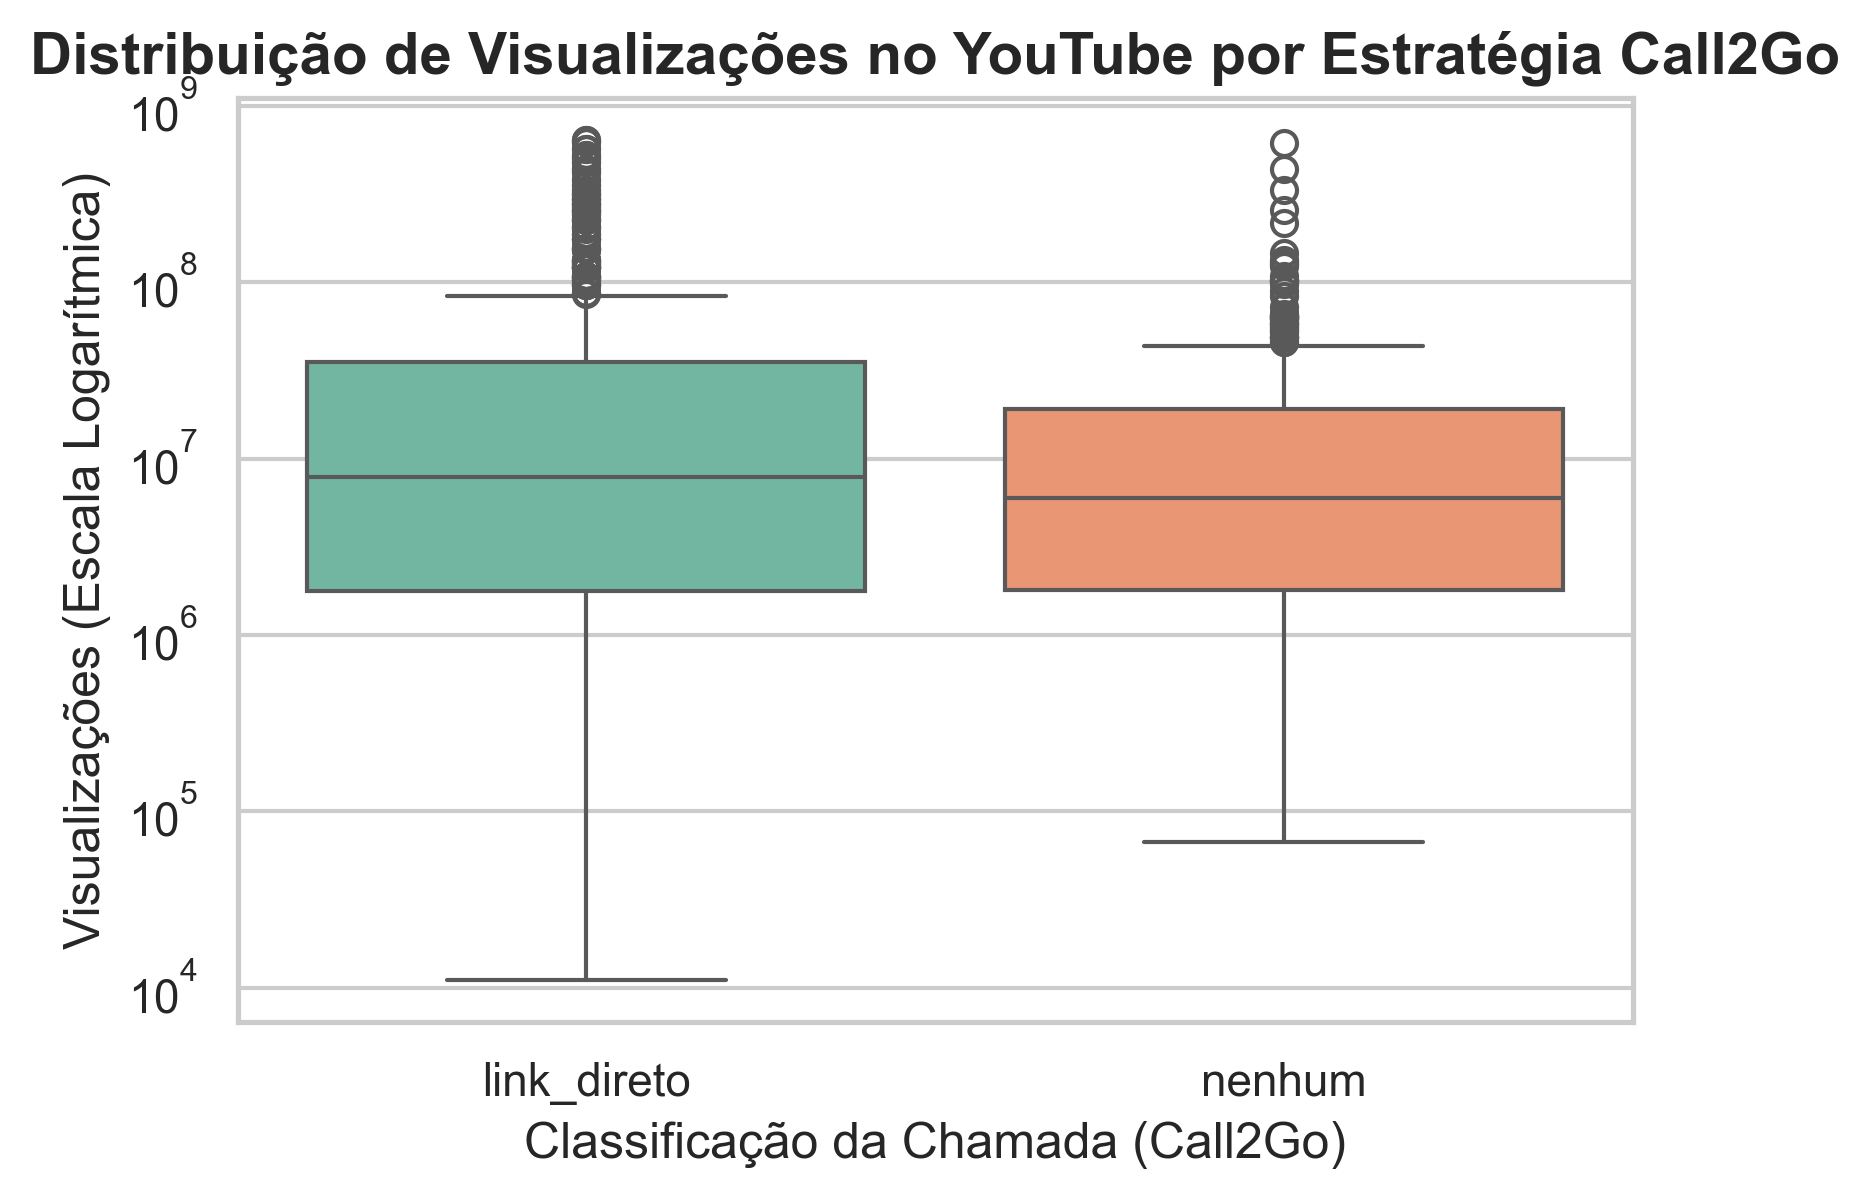
\includegraphics[width=.78\textwidth]{figs/boxplot_call2go_views.png}
\caption{Boxplot comparativo de visualizações (escala logarítmica) entre
vídeos com Call2Go~OR ($n=518$) e sem Call2Go ($n=1.123$). A diferença
descritiva de medianas não é estatisticamente significativa.}
\label{fig:boxplot}
\end{figure}

A diferença de medianas é descritivamente relevante, mas deve ser interpretada
com cautela: artistas de maior popularidade tendem simultaneamente a ter mais
visualizações \textbf{e} a adotar práticas profissionalizadas de marketing
(incluindo Call2Go), configurando uma variável confundidora que será abordada
pelos testes formais na subseção seguinte.

\subsection{Testes de Hipótese $H_2$ e $H_3$}

A Tabela~\ref{tab:hipoteses} sintetiza os resultados dos testes Mann-Whitney~U
para as hipóteses de impacto, reportados para as métricas OR (primária) e AND
(sub-análise).

\begin{table}[H]
\centering
\caption{Resultados Mann-Whitney~U para $H_2$ (visualizações YouTube) e
$H_3$ (popularidade Spotify), métricas OR e AND.}
\label{tab:hipoteses}
\renewcommand{\arraystretch}{1.2}
\begin{tabular}{@{}lllccc@{}}
\toprule
\textbf{Hipótese} & \textbf{Métrica} & \textbf{Grupos ($n$)} &
\textbf{$U$} & \textbf{$p$} & \textbf{Decisão} \\
\midrule
$H_2$: Call2Go $\to$ Views YT & OR  & $518$ vs $1.123$ & 280.705 & $0{,}872$ & $\neg H_0$ \\
$H_2$: Call2Go $\to$ Views YT & AND & $88$ vs $1.553$  & 73.010  & $0{,}140$ & $\neg H_0$ \\
$H_3$: Call2Go $\to$ Pop.\ SP & OR  & (join Spotify)   & ---     & $1{,}000$ & $\neg H_0$ \\
$H_3$: Call2Go $\to$ Pop.\ SP & AND & (join Spotify)   & ---     & $0{,}998$ & $\neg H_0$ \\
\bottomrule
\multicolumn{6}{@{}l@{}}{\footnotesize $\neg H_0$ = não rejeita $H_0$; $\alpha=0{,}05$;
SP = Spotify.}
\end{tabular}
\end{table}

Os resultados para $H_2$ (OR: $p = 0{,}872$; AND: $p = 0{,}140$) e para $H_3$
(OR: $p = 1{,}000$; AND: $p = 0{,}998$) levam à \textbf{não rejeição} da
hipótese nula em todos os cenários testados. A interpretação é que a diferença
de visualizações observada descritivamente não é estatisticamente distinguível
do esperado por acaso ao nível de 5\%, indicando que a popularidade geral do
artista---e não o Call2Go em si---explica tanto a maior quantidade de
visualizações quanto a adoção da estratégia.

\subsection{Análise Bidirecional YouTube $\leftrightarrow$ Spotify}

A dispersão \textit{cross-platform} (Figura~\ref{fig:heatmap}) e a
Tabela~\ref{tab:spearman} sumarizam os resultados da análise bidirecional.

\begin{table}[H]
\centering
\caption{Análise bidirecional de Spearman ($\alpha = 0{,}10$; $N = 67$
artistas).}
\label{tab:spearman}
\renewcommand{\arraystretch}{1.15}
\begin{tabular}{@{}llccc@{}}
\toprule
\textbf{Direção} & \textbf{Correlação} & \textbf{$\rho$} &
\textbf{$p$} & \textbf{Sig.} \\
\midrule
A (YT $\to$ SP) & Taxa Call2Go OR $\leftrightarrow$ Pop.\ Spotify
  & $0{,}008$ & $0{,}947$ & n.s. \\
A (YT $\to$ SP) & Taxa Call2Go OR $\leftrightarrow$ Seguidores SP
  & $0{,}019$ & $0{,}877$ & n.s. \\
\midrule
B (SP $\to$ YT) & Pop.\ Spotify $\leftrightarrow$ Média Views YT
  & $0{,}505$ & $< 0{,}001$ & *** \\
B (SP $\to$ YT) & Seguidores SP $\leftrightarrow$ Média Views YT
  & $0{,}674$ & $< 0{,}001$ & *** \\
\bottomrule
\multicolumn{5}{@{}l@{}}{\footnotesize *** $p<0{,}001$; n.s. = não
significativo; SP = Spotify; YT = YouTube.}
\end{tabular}
\end{table}

A análise bidirecional (Tabela~\ref{tab:spearman} e
Figura~\ref{fig:heatmap}) classifica a relação como
\textbf{unidirecional: Spotify~$\to$~YouTube}: todas as correlações da
Direção~B são fortemente significativas ($\rho = 0{,}505$, $p < 0{,}001$),
enquanto nenhuma correlação da Direção~A atinge significância. A relação
é correlacional, não causal.

\begin{figure}[H]
\centering
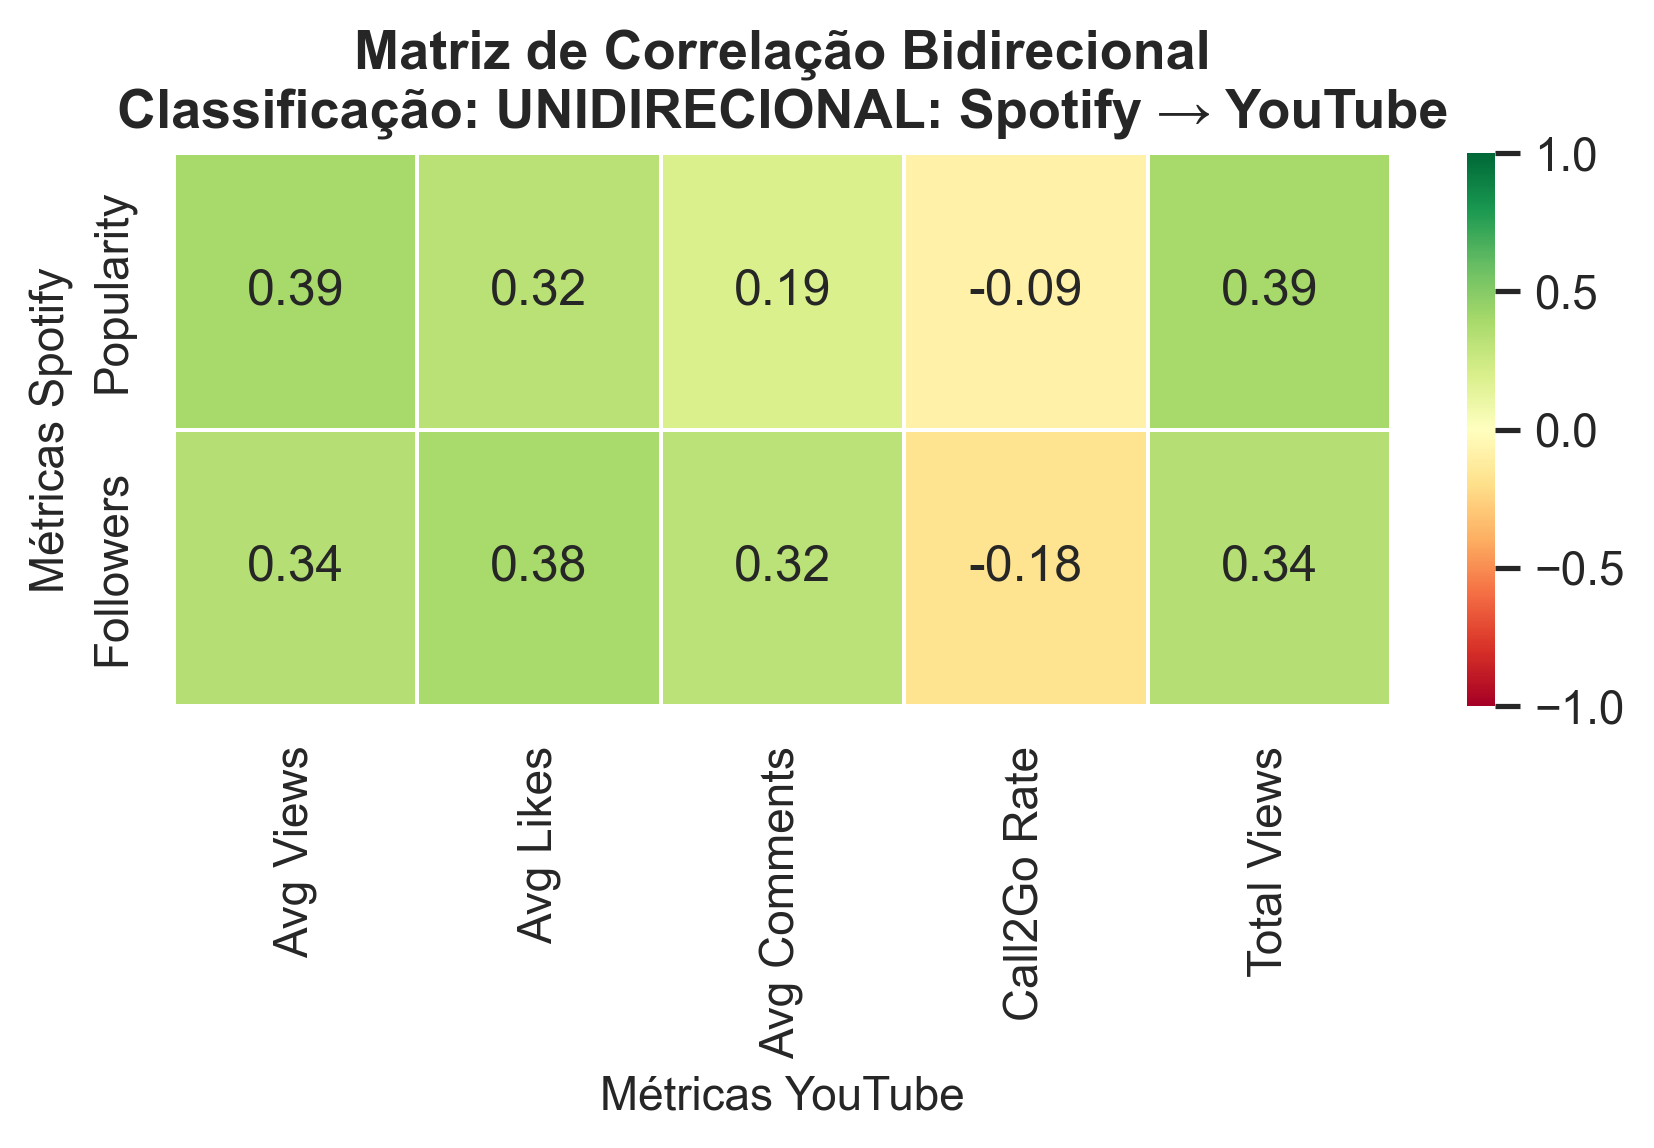
\includegraphics[width=.78\textwidth]{figs/bidirectional_correlation_matrix.png}
\caption{Matriz de correlação bidirecional (Spearman) entre métricas YouTube
e Spotify ($N = 67$ artistas). A assimetria entre as direções A e B evidencia
o efeito unidirecional Spotify~$\to$~YouTube.}
\label{fig:heatmap}
\end{figure}

\subsection{Análise Temporal: Defasagem YouTube \textit{vs.\ Charts} Spotify
($H_4$)}
\label{sec:temporal}

A análise temporal foi conduzida sobre os 39 artistas da base semente
identificados como primários nos \textit{charts} Q1~2026. A defasagem
(\textit{lag}) foi calculada como a diferença em dias entre a data do
primeiro vídeo do artista no YouTube e sua data de entrada no \textit{chart}
Spotify BR. Valores negativos indicam que o YouTube precedeu o
\textit{chart}; valores positivos indicariam o contrário.

A mediana de \texttt{lag\_any\_days} foi de \textbf{$-882$~dias}
(IQR: $[-1.814; -360]$), indicando que para 95\% dos artistas a atividade no
YouTube precede a entrada nos \textit{charts} em quase dois anos e meio. Para
os 18 artistas com Call2Go confirmado antes da entrada no \textit{chart}, a
mediana de \texttt{lag\_call2go\_days} foi de $-824$~dias
(IQR: $[-1.537; -296]$), com 89\% (16/18) tendo adotado Call2Go \textit{antes}
da estreia nos \textit{charts}.

\begin{figure}[H]
\centering
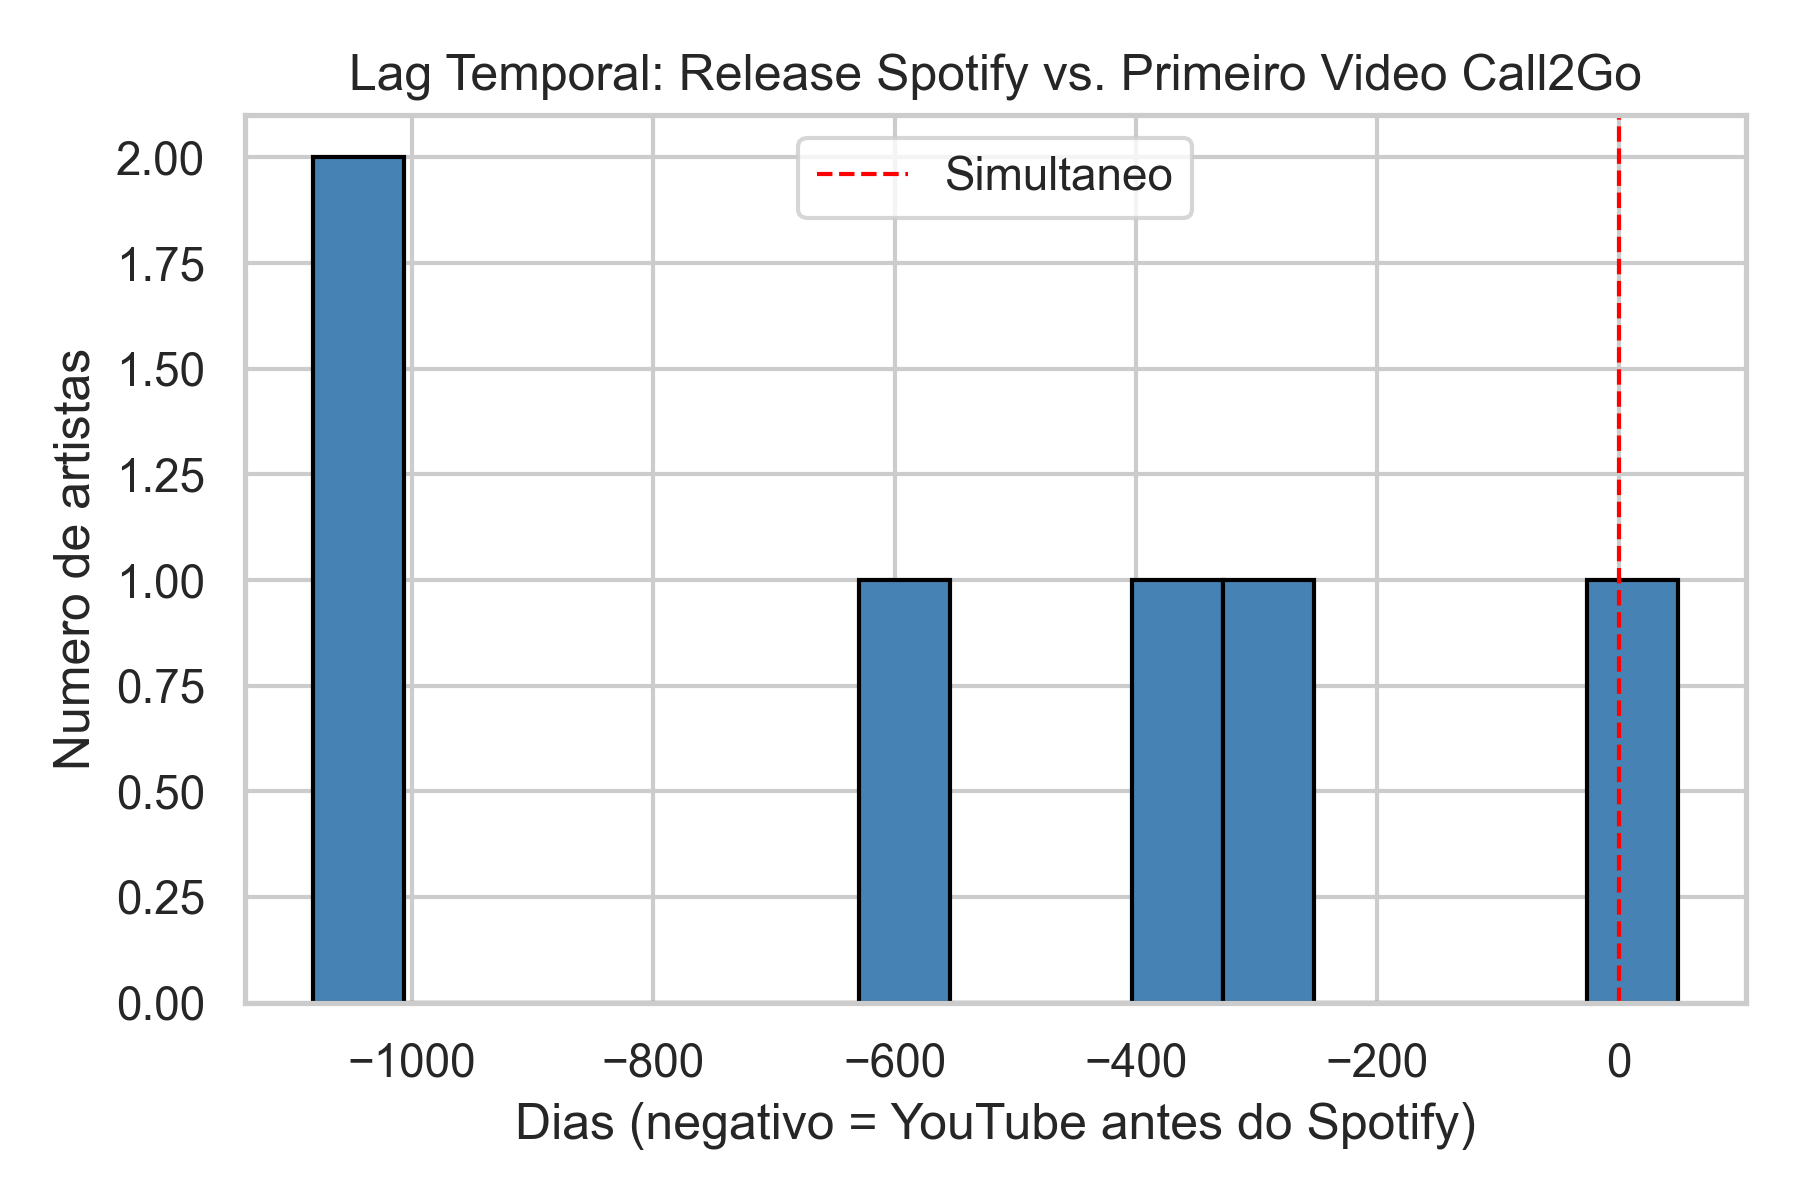
\includegraphics[width=.78\textwidth]{figs/temporal_lag_analysis.png}
\caption{Defasagem temporal (dias) entre a atividade no YouTube e a entrada
nos \textit{charts} Spotify BR ($n=39$ artistas). Valores negativos indicam
que o YouTube precede os \textit{charts}; a mediana de $-882$~dias demonstra
que o YouTube opera como palco de construção de reputação antecedente ao
sucesso nos \textit{charts}.}
\label{fig:temporal}
\end{figure}

A Tabela~\ref{tab:temporal} apresenta as correlações de Spearman entre as
janelas de atividade pré-entrada e o desempenho nos \textit{charts}.

\begin{table}[H]
\centering
\caption{Correlações de Spearman entre atividade YouTube pré-entrada e score
\textit{cross-platform} ($n=39$ artistas; $\alpha=0{,}05$).}
\label{tab:temporal}
\renewcommand{\arraystretch}{1.15}
\begin{tabular}{@{}llccc@{}}
\toprule
\textbf{Variável X (YouTube)} & \textbf{Variável Y (Charts)} &
\textbf{$\rho$} & \textbf{$p$} & \textbf{Sig.} \\
\midrule
Vídeos publicados nos 30d pré-chart & Score combinado      & $0{,}364$ & $0{,}022$ & * \\
\textit{Lag} Call2Go (dias)         & Score Spotify        & $0{,}028$ & $0{,}913$ & n.s. \\
Call2Go presente pré-chart (0/1)    & Score Spotify        & $-0{,}093$ & $0{,}575$ & n.s. \\
\bottomrule
\multicolumn{5}{@{}l@{}}{\footnotesize * $p<0{,}05$; n.s. = não significativo.}
\end{tabular}
\end{table}

O único preditor significativo identificado é o \textbf{volume de publicações
nos 30~dias anteriores à entrada no \textit{chart}} ($\rho = 0{,}364$,
$p = 0{,}022$): artistas que publicam mais vídeos no YouTube imediatamente
antes da estreia nos \textit{charts} tendem a apresentar maior
\textit{score} combinado \textit{cross-platform}. As métricas relacionadas
ao Call2Go especificamente não apresentaram correlação significativa com o
desempenho futuro nos \textit{charts}, resultado coerente com a ausência de
efeito encontrada em $H_2$ e $H_3$.

\subsection{Converg\^encia Multiplataforma e Auditoria de Voltas}

A integra\c{c}\~ao com o Last.fm revelou que apenas 9/67 artistas (13,4\%)
figuram simultaneamente no Top~200~BR Last.fm; a correla\c{c}\~ao Seguidores
Spotify~$\leftrightarrow$~Scrobbles Last.fm ($\rho = 0{,}848$, $p < 0{,}001$)
confirma consist\^encia entre plataformas. Testes sobre m\'etricas Last.fm
n\~ao identificaram efeito do Call2Go~OR em \textit{listeners} ($p = 0{,}865$),
\textit{scrobbles} ($p = 0{,}960$), presen\c{c}a nos \textit{charts}
($\chi^2 = 2{,}610$, $p = 0{,}106$) nem g\^enero ($\chi^2 = 2{,}293$,
$p = 0{,}682$). Esses resultados em fonte independente refor\c{c}am os
achados de $H_2$ e $H_3$. Uma auditoria via
Playwright~\cite{playwrightapi2024} verificou 0/67 links reversos em quatro
dire\c{c}\~oes (Spotify/Last.fm~$\to$~YouTube/Spotify), confirmando que o
fluxo Call2Go \'e estruturalmente unidirecional: YouTube~$\to$~Spotify.

\subsection{Validação Cruzada do Detector ($H_0$/$H_1$)}

A Tabela~\ref{tab:crossval} apresenta as métricas de confiabilidade do
detector obtidas sobre os 91 vídeos adversariais com anotação às cegas.

\begin{table}[H]
\centering
\caption{Métricas de confiabilidade do detector (validação adversarial:
91 vídeos, anotação às cegas, IC~95\% \textit{bootstrap}).}
\label{tab:crossval}
\renewcommand{\arraystretch}{1.2}
\begin{tabular}{@{}lcccl@{}}
\toprule
\textbf{Nível} & \textbf{Acurácia} & \textbf{Kappa ($\kappa$)} &
\textbf{Interpretação} & \textbf{Decisão $H_0$} \\
\midrule
Vídeo & 82,4\% & 0,45 & Moderado   & Não rejeita $H_0$ ($<85\%$) \\
\textbf{Canal} & \textbf{90,1\%} & \textbf{0,80} & \textbf{Substancial} &
\textbf{Rejeita $H_0$ ($\geq 85\%$)} \\
\bottomrule
\multicolumn{5}{@{}l@{}}{\footnotesize Escala Landis \& Koch~\cite{landis1977}:
$0{,}61$--$0{,}80$ = substancial; $0{,}41$--$0{,}60$ = moderado.}
\end{tabular}
\end{table}

Os resultados confirmam que o sistema opera de forma satisfatória para os fins
deste estudo. \textbf{Nível canal}: $\kappa = 0{,}80$ (substancial) e acurácia
de 90,1\% rejeitam $H_0$, validando o uso do detector como ferramenta
analítica. Os resultados da anotação manual foram utilizados como parâmetro
para atestar a confiabilidade do sistema e dar continuidade às análises.
\textbf{Nível vídeo}: $\kappa = 0{,}45$ (moderado) e acurácia de 82,4\% não
rejeitam $H_0$. O resultado é esperado: artistas frequentemente inserem o
Call2Go apenas no perfil do canal, não em cada descrição de vídeo. A métrica
OR, que combina os dois níveis, compensa essa limitação e constitui o modo
de operação adotado nas análises subsequentes.

% ============================================================
%  6. CONCLUSÕES E TRABALHOS FUTUROS
% ============================================================
\section{Conclusões e Trabalhos Futuros}
\label{sec:conclusao}

Este trabalho apresentou, implementou e avaliou um sistema automatizado para
detecção de estratégias Call2Go em vídeos do YouTube, aplicado a um corpus
de 1.641 vídeos de 67 artistas brasileiros persistentes \textit{cross-platform}
nos \textit{charts} Q1~2026. Os principais achados são sintetizados a seguir.

\textbf{Confiabilidade do detector ($H_0$/$H_1$):} a validação adversarial
às cegas com 91 vídeos revelou $\kappa = 0{,}80$ no nível canal (substancial;
acurácia 90,1\%), rejeitando $H_0$ para esse nível e validando a abordagem.
No nível vídeo, $\kappa = 0{,}45$ e acurácia 82,4\% não rejeitam $H_0$,
evidenciando a limitação do detector isolado na descrição individual---e
justificando a arquitetura bicamada com operador OR como modo primário de
operação. O sistema demonstra comportamento determinístico, interpretável e
auditável, com seis iterações de correção de bugs documentadas.

\textbf{Impacto no engajamento ($H_2$ e $H_3$):} os testes Mann-Whitney~U
não encontraram evidências de impacto significativo do Call2Go nas
visualizações do YouTube (OR: $p = 0{,}872$) nem na popularidade do Spotify
(OR: $p = 1{,}000$), para nenhuma das métricas testadas. O padrão é coerente
em três plataformas independentes (YouTube, Spotify e Last.fm), sugerindo que
o Call2Go está associado à popularidade geral do artista---variável
confundidora---e não a um efeito isolado da estratégia.

\textbf{Direcionalidade \textit{cross-platform}:} a análise bidirecional
confirmou efeito unidirecional Spotify~$\to$~YouTube ($\rho = 0{,}505$,
$p < 0{,}001$). Artistas com maior presença no Spotify acumulam mais
visualizações no YouTube; o inverso não se sustenta estatisticamente. A
auditoria automatizada (Playwright, 67 artistas, 4 direções) confirmou a
ausência de links reversos, reforçando a assimetria estrutural do ecossistema.

\textbf{Análise temporal ($H_4$):} o YouTube precede a entrada nos
\textit{charts} Spotify em mediana de 882~dias para 95\% dos artistas,
sugerindo que a plataforma de vídeo opera como palco de construção de
reputação antecedente ao sucesso nos \textit{charts}. O único preditor
significativo identificado foi o volume de publicações nos 30~dias
pré-entrada ($\rho = 0{,}364$, $p = 0{,}022$), indicando que a intensidade
de publicação imediatamente antes da estreia nos \textit{charts} reflete---e
possivelmente contribui para---a projeção \textit{cross-platform} do artista.

\textbf{Contribuições metodológicas:} o pipeline ETL de 15 etapas é
inteiramente reprodutível, executável a partir de estado limpo em 39,9
segundos, produzindo 30 artefatos determinísticos. O design adversarial do
protocolo de validação, com anotação às cegas, representa melhoria
metodológica em relação a abordagens circulares. A integração de três
plataformas (YouTube, Spotify e Last.fm) e de dados de \textit{charts}
semanais Q1~2026 permite análises de convergência não disponíveis em trabalhos
que operam com plataformas isoladas.

\textbf{Limitações:} (i)~o corpus é limitado ao segmento de artistas de alta
visibilidade; a metodologia de detecção é transferível, mas os achados
empíricos não se generalizam diretamente para artistas independentes;
(ii)~as métricas do Spotify constituem \textit{snapshot} transversal, sem
seriação temporal, impedindo análise de causalidade; (iii)~o campo
\texttt{popularity} do Spotify é opaco---a fórmula exata de cálculo não é
pública; (iv)~o Kappa de vídeo (0,45) indica margem de melhoria no detector
a nível de descrição individual, possível com regras adicionais ou com
modelos de NLP.

\textbf{Trabalhos futuros:} a análise temporal poderia ser enriquecida com
dados longitudinais de \textit{streams} semanais no Spotify, permitindo
modelagem de causalidade de Granger. O sistema de detecção pode ser estendido
com modelos de linguagem (\textit{transformers}) para CTAs em formatos não
estruturados. A metodologia do pipeline é transferível para outros pares de
plataformas (e.g., TikTok~$\to$~Spotify ou Instagram~$\to$~YouTube), e a
base de artistas persistentes Q1~2026 pode ser atualizada trimestralmente
para análises longitudinais de adoção da estratégia.

% ============================================================
%  REFERÊNCIAS
% ============================================================
\bibliographystyle{sbc}
\bibliography{references}

\end{document}
